\section{Crowd plug-in}

The goal of this work package was to implement and integrate into
Blender an efficient and realistic motion of a crowd . At first we
wanted to implement a general movement algorithm and an other
algorithm that would control the animation of the crowd. The second
part was quite difficult to implement and thus we decided to
concentrate ourselves on the first part.



The initial goal was to implement two parts: one creating trajectories
for the crowd and another one for animating individual movements. The
second part was really hard to implement and was closely linked with
the animation of models, which is a domain where we did not have any
expertise. We thus decided to focus on the first part.


Our code is split into two parts: one that is independent from Blender
and one that depends on it (see figure \ref{fig:code}).


The first part create a set of key points that will represent the
movement of one person and the second interpolate a trajectory from
those points. Before presenting these two parts, we explain the
difficulties encountered when we tried to model human animation.


\subsection{Human animation}

At the beginning we considered animating Humans and started by
analyzing a theoretical survey of computer animation of Human walking
(\cite{th_walking}) and looking for what was already done in Blender
concerning automatic walking. All Blender-related resources on walking
animation are gathered on a web-page
(\cite{blwikiwalking}). Walk-o-matic and stride add-ons were used in
previous versions of Blender to ``help to interactively design rough
passes of a walk'' and ``quickly create cycles for background or extra
characters'', however both were broken on Blender 2.7 and we are using
Blender 2.76.

Due to the lack of existing tools concerning automatic walking we
considered creating such a tool ourselves. We started by analyzing
tutorials on blender character animation (for example
\cite{tuto_walk}) and creating such a motion manually. However we soon
realized how difficult it is to generate a realistic walk due to the
complex physics behind the movements and decided that it is out of the
scope of our project. We have shifted our attention to the more basic
task of creating a path in Blender and making an object following it
with varying speed given by our algorithm.


% Il faudra changer les titres je pense %% bon il faut peut être encore les changer
\subsection{Path generation}

The first algorithm is inspired by those two papers: \cite{PLE} and
\cite{vandenBerg2011}. We chose them because it relied on graphs
rather than cellular automaton, and we were more familiar with
graphs. We also thought this approach would be more precise.

% TODO :combler avec du bla bla

The idea is the following: a graph (grid) algorithm will generate a
general path for each individual and another algorithm will prevent
collisions between individuals.


Time is discretized, and for each time, we compute the direction to go
for each individual. We move the in this direction, and iterate this
principle. This is how we get the final set of points for each
individuals.


\subsubsection{Implementation}

%% Expliquer les parties avant de se lancer ?

\paragraph{The guide graph}

The first part that we tried to implement was the data structure of
the graph. We created a data structure representing the nodes of the
graph and the edges. This was quite easy to do since the graph is
supposed to be a grid, it is regular.  Then we needed a minimum
distance (1 to 1) algorithm on the graph. For that we chose the $A^*$
algorithm. Unfortunately, our implementation of the $A^*$ was really
costly in time and even more in memory. This fact forced us to abandon
the graph in the rest of the development. We could test it for small
values, and for a small number of calls, but the $A^*$ procedure would
have to be called thousands of times which makes this impractical.  To
replace the graph we used the euclidean distance, but we had to remove
 static obstacles. Indeed these obstacles were taken into
account in the graph (no vertices inside an obstacle) and impacted the
shortest path algorithm $A^*$ but euclidean distance cannot take into
account such obstacles.
Also the points (representing people) were not able to avoid packed
places anymore and just went strait to there goal, same as for obstacles,
packed places were taken into account by the edges of the graph which weigth
depended on the crowdedness of the neighbour cells.

\begin{figure}[h!]
  \centering
  \begin{subfigure}[t]{0.45\textwidth}
    \scalebox{.4}{% Graphic for TeX using PGF
% Title: /home/johanna/Documents/Informatique/M1/Projet/pib/beamer_final/short_path.dia
% Creator: Dia v0.97.3
% CreationDate: Wed Apr 13 17:17:40 2016
% For: johanna
% \usepackage{tikz}
% The following commands are not supported in PSTricks at present
% We define them conditionally, so when they are implemented,
% this pgf file will use them.
\ifx\du\undefined
  \newlength{\du}
\fi
\setlength{\du}{15\unitlength}
\begin{tikzpicture}
\pgftransformxscale{1.000000}
\pgftransformyscale{-1.000000}
\definecolor{dialinecolor}{rgb}{0.000000, 0.000000, 0.000000}
\pgfsetstrokecolor{dialinecolor}
\definecolor{dialinecolor}{rgb}{1.000000, 1.000000, 1.000000}
\pgfsetfillcolor{dialinecolor}
\pgfsetlinewidth{0.200000\du}
\pgfsetdash{}{0pt}
\pgfsetdash{}{0pt}
\pgfsetbuttcap
{
\definecolor{dialinecolor}{rgb}{0.000000, 0.000000, 0.000000}
\pgfsetfillcolor{dialinecolor}
% was here!!!
\definecolor{dialinecolor}{rgb}{0.000000, 0.000000, 0.000000}
\pgfsetstrokecolor{dialinecolor}
\draw (45.000000\du,-13.000000\du)--(75.000000\du,-10.000000\du);
}
\pgfsetlinewidth{0.200000\du}
\pgfsetdash{}{0pt}
\pgfsetdash{}{0pt}
\pgfsetmiterjoin
\pgfsetbuttcap
{
\definecolor{dialinecolor}{rgb}{0.000000, 0.000000, 0.000000}
\pgfsetfillcolor{dialinecolor}
% was here!!!
\definecolor{dialinecolor}{rgb}{0.000000, 0.000000, 0.000000}
\pgfsetstrokecolor{dialinecolor}
\pgfpathmoveto{\pgfpoint{75.000000\du}{-10.000000\du}}
\pgfpathcurveto{\pgfpoint{77.000000\du}{-4.000000\du}}{\pgfpoint{77.000000\du}{6.000000\du}}{\pgfpoint{77.000000\du}{6.000000\du}}
\pgfusepath{stroke}
}
\pgfsetlinewidth{0.200000\du}
\pgfsetdash{}{0pt}
\pgfsetdash{}{0pt}
\pgfsetbuttcap
{
\definecolor{dialinecolor}{rgb}{0.000000, 0.000000, 0.000000}
\pgfsetfillcolor{dialinecolor}
% was here!!!
\definecolor{dialinecolor}{rgb}{0.000000, 0.000000, 0.000000}
\pgfsetstrokecolor{dialinecolor}
\draw (50.000000\du,-7.000000\du)--(70.000000\du,-5.000000\du);
}
\pgfsetlinewidth{0.200000\du}
\pgfsetdash{}{0pt}
\pgfsetdash{}{0pt}
\pgfsetbuttcap
{
\definecolor{dialinecolor}{rgb}{0.000000, 0.000000, 0.000000}
\pgfsetfillcolor{dialinecolor}
% was here!!!
\definecolor{dialinecolor}{rgb}{0.000000, 0.000000, 0.000000}
\pgfsetstrokecolor{dialinecolor}
\draw (70.000000\du,-5.000000\du)--(70.000000\du,2.000000\du);
}
\pgfsetlinewidth{0.200000\du}
\pgfsetdash{}{0pt}
\pgfsetdash{}{0pt}
\pgfsetmiterjoin
\pgfsetbuttcap
{
\definecolor{dialinecolor}{rgb}{0.000000, 0.000000, 0.000000}
\pgfsetfillcolor{dialinecolor}
% was here!!!
\definecolor{dialinecolor}{rgb}{0.000000, 0.000000, 0.000000}
\pgfsetstrokecolor{dialinecolor}
\pgfpathmoveto{\pgfpoint{50.000000\du}{-7.000000\du}}
\pgfpathcurveto{\pgfpoint{50.000000\du}{2.000000\du}}{\pgfpoint{67.676000\du}{2.000000\du}}{\pgfpoint{70.000000\du}{2.000000\du}}
\pgfusepath{stroke}
}
\pgfsetlinewidth{0.200000\du}
\pgfsetdash{}{0pt}
\pgfsetdash{}{0pt}
\pgfsetbuttcap
\pgfsetmiterjoin
\pgfsetlinewidth{0.200000\du}
\pgfsetbuttcap
\pgfsetmiterjoin
\pgfsetdash{}{0pt}
\definecolor{dialinecolor}{rgb}{1.000000, 1.000000, 1.000000}
\pgfsetfillcolor{dialinecolor}
\fill (72.000000\du,-7.000000\du)--(72.750000\du,-7.250000\du)--(73.000000\du,-8.000000\du)--(73.250000\du,-7.250000\du)--(74.000000\du,-7.000000\du)--(73.250000\du,-6.750000\du)--(73.000000\du,-6.000000\du)--(72.750000\du,-6.750000\du)--cycle;
\definecolor{dialinecolor}{rgb}{0.000000, 0.000000, 0.000000}
\pgfsetstrokecolor{dialinecolor}
\draw (72.000000\du,-7.000000\du)--(72.750000\du,-7.250000\du)--(73.000000\du,-8.000000\du)--(73.250000\du,-7.250000\du)--(74.000000\du,-7.000000\du)--(73.250000\du,-6.750000\du)--(73.000000\du,-6.000000\du)--(72.750000\du,-6.750000\du)--cycle;
\pgfsetbuttcap
\pgfsetmiterjoin
\pgfsetdash{}{0pt}
\definecolor{dialinecolor}{rgb}{0.000000, 0.000000, 0.000000}
\pgfsetstrokecolor{dialinecolor}
\draw (72.000000\du,-7.000000\du)--(72.750000\du,-7.250000\du)--(73.000000\du,-8.000000\du)--(73.250000\du,-7.250000\du)--(74.000000\du,-7.000000\du)--(73.250000\du,-6.750000\du)--(73.000000\du,-6.000000\du)--(72.750000\du,-6.750000\du)--cycle;
\pgfsetlinewidth{0.200000\du}
\pgfsetdash{}{0pt}
\pgfsetdash{}{0pt}
\pgfsetbuttcap
\pgfsetmiterjoin
\pgfsetlinewidth{0.200000\du}
\pgfsetbuttcap
\pgfsetmiterjoin
\pgfsetdash{}{0pt}
\definecolor{dialinecolor}{rgb}{1.000000, 1.000000, 1.000000}
\pgfsetfillcolor{dialinecolor}
\fill (47.500000\du,-10.499997\du)--(48.000000\du,-9.499997\du)--(47.000000\du,-9.499997\du)--cycle;
\definecolor{dialinecolor}{rgb}{1.000000, 0.027451, 0.027451}
\pgfsetstrokecolor{dialinecolor}
\draw (47.500000\du,-10.499997\du)--(48.000000\du,-9.499997\du)--(47.000000\du,-9.499997\du)--cycle;
\pgfsetlinewidth{0.200000\du}
\pgfsetdash{}{0pt}
\pgfsetdash{}{0pt}
\pgfsetbuttcap
\pgfsetmiterjoin
\pgfsetlinewidth{0.200000\du}
\pgfsetbuttcap
\pgfsetmiterjoin
\pgfsetdash{}{0pt}
\definecolor{dialinecolor}{rgb}{1.000000, 1.000000, 1.000000}
\pgfsetfillcolor{dialinecolor}
\fill (56.500000\du,-8.000000\du)--(57.000000\du,-7.000000\du)--(56.000000\du,-7.000000\du)--cycle;
\definecolor{dialinecolor}{rgb}{0.000000, 0.000000, 0.000000}
\pgfsetstrokecolor{dialinecolor}
\draw (56.500000\du,-8.000000\du)--(57.000000\du,-7.000000\du)--(56.000000\du,-7.000000\du)--cycle;
\pgfsetlinewidth{0.200000\du}
\pgfsetdash{}{0pt}
\pgfsetdash{}{0pt}
\pgfsetbuttcap
\pgfsetmiterjoin
\pgfsetlinewidth{0.200000\du}
\pgfsetbuttcap
\pgfsetmiterjoin
\pgfsetdash{}{0pt}
\definecolor{dialinecolor}{rgb}{1.000000, 1.000000, 1.000000}
\pgfsetfillcolor{dialinecolor}
\fill (56.500000\du,-11.000000\du)--(57.000000\du,-10.000000\du)--(56.000000\du,-10.000000\du)--cycle;
\definecolor{dialinecolor}{rgb}{0.000000, 0.000000, 0.000000}
\pgfsetstrokecolor{dialinecolor}
\draw (56.500000\du,-11.000000\du)--(57.000000\du,-10.000000\du)--(56.000000\du,-10.000000\du)--cycle;
\pgfsetlinewidth{0.200000\du}
\pgfsetdash{}{0pt}
\pgfsetdash{}{0pt}
\pgfsetbuttcap
\pgfsetmiterjoin
\pgfsetlinewidth{0.200000\du}
\pgfsetbuttcap
\pgfsetmiterjoin
\pgfsetdash{}{0pt}
\definecolor{dialinecolor}{rgb}{1.000000, 1.000000, 1.000000}
\pgfsetfillcolor{dialinecolor}
\fill (59.500000\du,-11.000000\du)--(60.000000\du,-10.000000\du)--(59.000000\du,-10.000000\du)--cycle;
\definecolor{dialinecolor}{rgb}{0.000000, 0.000000, 0.000000}
\pgfsetstrokecolor{dialinecolor}
\draw (59.500000\du,-11.000000\du)--(60.000000\du,-10.000000\du)--(59.000000\du,-10.000000\du)--cycle;
\pgfsetlinewidth{0.200000\du}
\pgfsetdash{}{0pt}
\pgfsetdash{}{0pt}
\pgfsetbuttcap
\pgfsetmiterjoin
\pgfsetlinewidth{0.200000\du}
\pgfsetbuttcap
\pgfsetmiterjoin
\pgfsetdash{}{0pt}
\definecolor{dialinecolor}{rgb}{1.000000, 1.000000, 1.000000}
\pgfsetfillcolor{dialinecolor}
\fill (59.500000\du,-8.000000\du)--(60.000000\du,-7.000000\du)--(59.000000\du,-7.000000\du)--cycle;
\definecolor{dialinecolor}{rgb}{0.000000, 0.000000, 0.000000}
\pgfsetstrokecolor{dialinecolor}
\draw (59.500000\du,-8.000000\du)--(60.000000\du,-7.000000\du)--(59.000000\du,-7.000000\du)--cycle;
\pgfsetlinewidth{0.200000\du}
\pgfsetdash{}{0pt}
\pgfsetdash{}{0pt}
\pgfsetbuttcap
\pgfsetmiterjoin
\pgfsetlinewidth{0.200000\du}
\pgfsetbuttcap
\pgfsetmiterjoin
\pgfsetdash{}{0pt}
\definecolor{dialinecolor}{rgb}{1.000000, 1.000000, 1.000000}
\pgfsetfillcolor{dialinecolor}
\fill (62.500000\du,-10.000000\du)--(63.000000\du,-9.000000\du)--(62.000000\du,-9.000000\du)--cycle;
\definecolor{dialinecolor}{rgb}{0.000000, 0.000000, 0.000000}
\pgfsetstrokecolor{dialinecolor}
\draw (62.500000\du,-10.000000\du)--(63.000000\du,-9.000000\du)--(62.000000\du,-9.000000\du)--cycle;
\pgfsetlinewidth{0.200000\du}
\pgfsetdash{}{0pt}
\pgfsetdash{}{0pt}
\pgfsetbuttcap
\pgfsetmiterjoin
\pgfsetlinewidth{0.200000\du}
\pgfsetbuttcap
\pgfsetmiterjoin
\pgfsetdash{}{0pt}
\definecolor{dialinecolor}{rgb}{1.000000, 1.000000, 1.000000}
\pgfsetfillcolor{dialinecolor}
\fill (62.500000\du,-7.000000\du)--(63.000000\du,-6.000000\du)--(62.000000\du,-6.000000\du)--cycle;
\definecolor{dialinecolor}{rgb}{0.000000, 0.000000, 0.000000}
\pgfsetstrokecolor{dialinecolor}
\draw (62.500000\du,-7.000000\du)--(63.000000\du,-6.000000\du)--(62.000000\du,-6.000000\du)--cycle;
\pgfsetlinewidth{0.200000\du}
\pgfsetdash{}{0pt}
\pgfsetdash{}{0pt}
\pgfsetbuttcap
\pgfsetmiterjoin
\pgfsetlinewidth{0.200000\du}
\pgfsetbuttcap
\pgfsetmiterjoin
\pgfsetdash{}{0pt}
\definecolor{dialinecolor}{rgb}{1.000000, 1.000000, 1.000000}
\pgfsetfillcolor{dialinecolor}
\fill (65.500000\du,-10.000000\du)--(66.000000\du,-9.000000\du)--(65.000000\du,-9.000000\du)--cycle;
\definecolor{dialinecolor}{rgb}{0.000000, 0.000000, 0.000000}
\pgfsetstrokecolor{dialinecolor}
\draw (65.500000\du,-10.000000\du)--(66.000000\du,-9.000000\du)--(65.000000\du,-9.000000\du)--cycle;
\pgfsetlinewidth{0.200000\du}
\pgfsetdash{}{0pt}
\pgfsetdash{}{0pt}
\pgfsetbuttcap
\pgfsetmiterjoin
\pgfsetlinewidth{0.200000\du}
\pgfsetbuttcap
\pgfsetmiterjoin
\pgfsetdash{}{0pt}
\definecolor{dialinecolor}{rgb}{1.000000, 1.000000, 1.000000}
\pgfsetfillcolor{dialinecolor}
\fill (64.500000\du,-7.000000\du)--(65.000000\du,-6.000000\du)--(64.000000\du,-6.000000\du)--cycle;
\definecolor{dialinecolor}{rgb}{0.000000, 0.000000, 0.000000}
\pgfsetstrokecolor{dialinecolor}
\draw (64.500000\du,-7.000000\du)--(65.000000\du,-6.000000\du)--(64.000000\du,-6.000000\du)--cycle;
\pgfsetlinewidth{0.200000\du}
\pgfsetdash{}{0pt}
\pgfsetdash{}{0pt}
\pgfsetbuttcap
\pgfsetmiterjoin
\pgfsetlinewidth{0.200000\du}
\pgfsetbuttcap
\pgfsetmiterjoin
\pgfsetdash{}{0pt}
\definecolor{dialinecolor}{rgb}{1.000000, 1.000000, 1.000000}
\pgfsetfillcolor{dialinecolor}
\fill (61.500000\du,-11.000000\du)--(62.000000\du,-10.000000\du)--(61.000000\du,-10.000000\du)--cycle;
\definecolor{dialinecolor}{rgb}{0.000000, 0.000000, 0.000000}
\pgfsetstrokecolor{dialinecolor}
\draw (61.500000\du,-11.000000\du)--(62.000000\du,-10.000000\du)--(61.000000\du,-10.000000\du)--cycle;
\end{tikzpicture}
}
    \caption{A setting in a crowd animation}
  \end{subfigure} % ~
  \begin{subfigure}[t]{0.45\textwidth}
    \scalebox{.4}{% Graphic for TeX using PGF
% Title: /home/johanna/Documents/Informatique/M1/Projet/pib/beamer_final/short_path_grid.dia
% Creator: Dia v0.97.3
% CreationDate: Wed Apr 13 20:23:16 2016
% For: johanna
% \usepackage{tikz}
% The following commands are not supported in PSTricks at present
% We define them conditionally, so when they are implemented,
% this pgf file will use them.
\ifx\du\undefined
  \newlength{\du}
\fi
\setlength{\du}{15\unitlength}
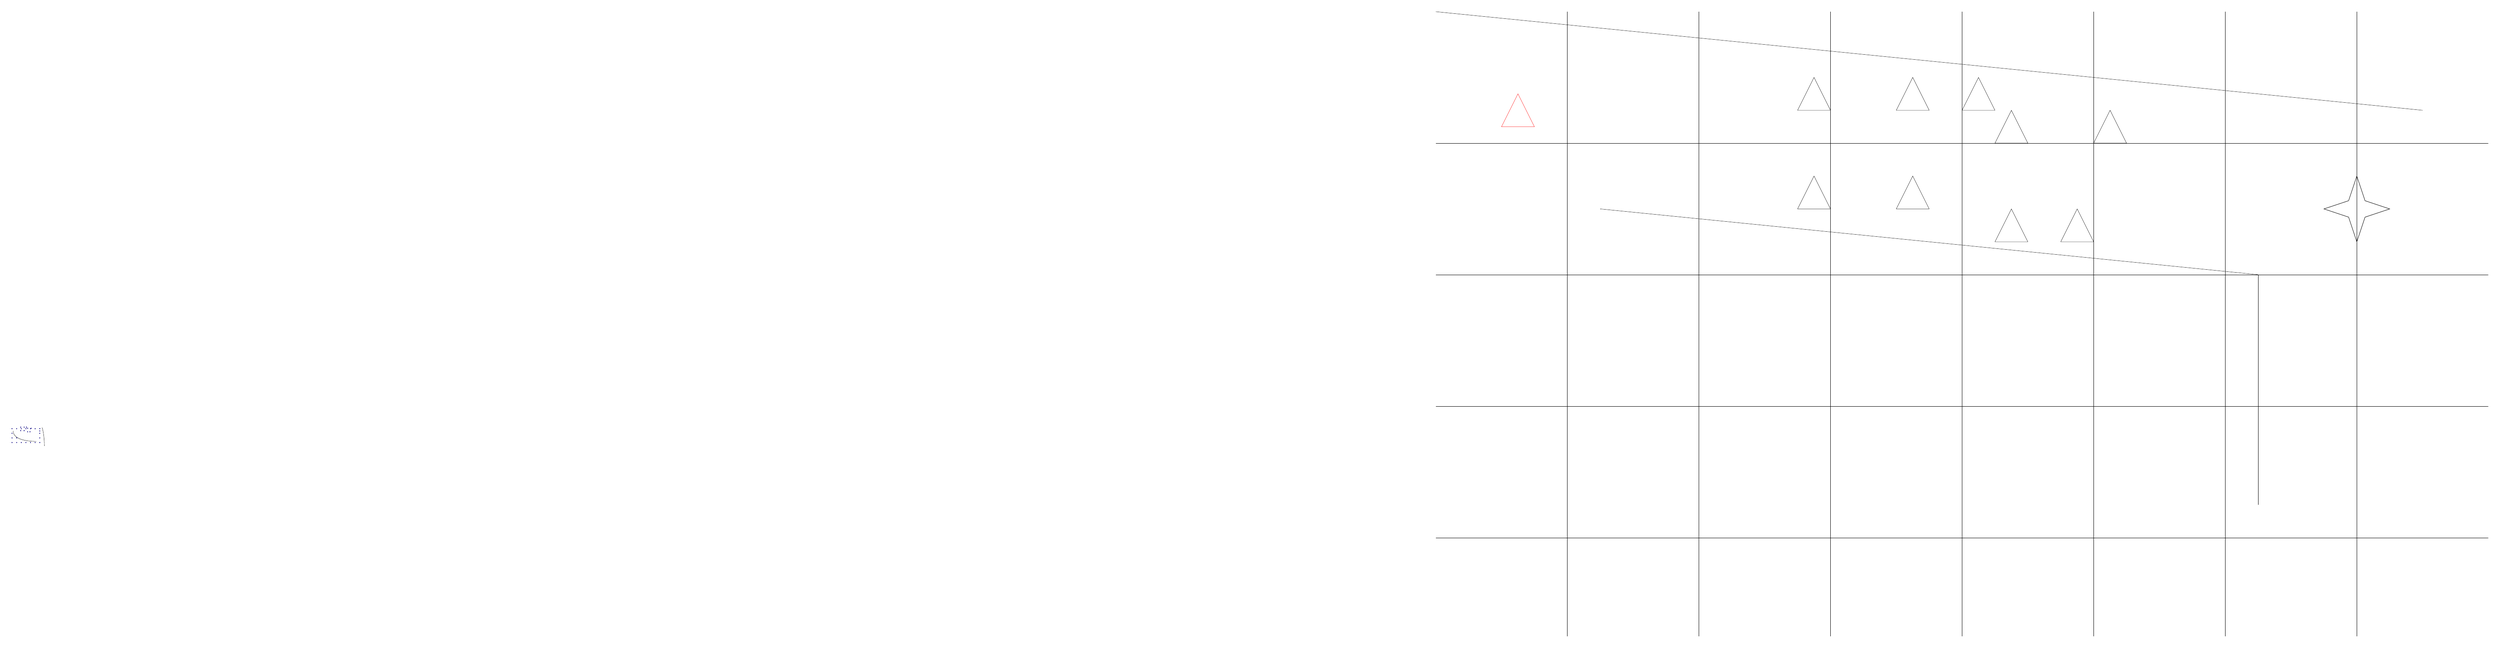
\begin{tikzpicture}
\pgftransformxscale{1.000000}
\pgftransformyscale{-1.000000}
\definecolor{dialinecolor}{rgb}{0.000000, 0.000000, 0.000000}
\pgfsetstrokecolor{dialinecolor}
\definecolor{dialinecolor}{rgb}{1.000000, 1.000000, 1.000000}
\pgfsetfillcolor{dialinecolor}
\pgfsetlinewidth{0.200000\du}
\pgfsetdash{}{0pt}
\pgfsetdash{}{0pt}
\pgfsetbuttcap
{
\definecolor{dialinecolor}{rgb}{0.000000, 0.000000, 0.000000}
\pgfsetfillcolor{dialinecolor}
% was here!!!
\definecolor{dialinecolor}{rgb}{0.000000, 0.000000, 0.000000}
\pgfsetstrokecolor{dialinecolor}
\draw (45.000000\du,-13.000000\du)--(75.000000\du,-10.000000\du);
}
\pgfsetlinewidth{0.200000\du}
\pgfsetdash{}{0pt}
\pgfsetdash{}{0pt}
\pgfsetmiterjoin
\pgfsetbuttcap
{
\definecolor{dialinecolor}{rgb}{0.000000, 0.000000, 0.000000}
\pgfsetfillcolor{dialinecolor}
% was here!!!
\definecolor{dialinecolor}{rgb}{0.000000, 0.000000, 0.000000}
\pgfsetstrokecolor{dialinecolor}
\pgfpathmoveto{\pgfpoint{75.000000\du}{-10.000000\du}}
\pgfpathcurveto{\pgfpoint{77.000000\du}{-4.000000\du}}{\pgfpoint{77.000000\du}{6.000000\du}}{\pgfpoint{77.000000\du}{6.000000\du}}
\pgfusepath{stroke}
}
\pgfsetlinewidth{0.200000\du}
\pgfsetdash{}{0pt}
\pgfsetdash{}{0pt}
\pgfsetbuttcap
{
\definecolor{dialinecolor}{rgb}{0.000000, 0.000000, 0.000000}
\pgfsetfillcolor{dialinecolor}
% was here!!!
\definecolor{dialinecolor}{rgb}{0.000000, 0.000000, 0.000000}
\pgfsetstrokecolor{dialinecolor}
\draw (50.000000\du,-7.000000\du)--(70.000000\du,-5.000000\du);
}
\pgfsetlinewidth{0.200000\du}
\pgfsetdash{}{0pt}
\pgfsetdash{}{0pt}
\pgfsetbuttcap
{
\definecolor{dialinecolor}{rgb}{0.000000, 0.000000, 0.000000}
\pgfsetfillcolor{dialinecolor}
% was here!!!
\definecolor{dialinecolor}{rgb}{0.000000, 0.000000, 0.000000}
\pgfsetstrokecolor{dialinecolor}
\draw (70.000000\du,-5.000000\du)--(70.000000\du,2.000000\du);
}
\pgfsetlinewidth{0.200000\du}
\pgfsetdash{}{0pt}
\pgfsetdash{}{0pt}
\pgfsetmiterjoin
\pgfsetbuttcap
{
\definecolor{dialinecolor}{rgb}{0.000000, 0.000000, 0.000000}
\pgfsetfillcolor{dialinecolor}
% was here!!!
\definecolor{dialinecolor}{rgb}{0.000000, 0.000000, 0.000000}
\pgfsetstrokecolor{dialinecolor}
\pgfpathmoveto{\pgfpoint{50.000000\du}{-7.000000\du}}
\pgfpathcurveto{\pgfpoint{50.000000\du}{2.000000\du}}{\pgfpoint{67.676000\du}{2.000000\du}}{\pgfpoint{70.000000\du}{2.000000\du}}
\pgfusepath{stroke}
}
\pgfsetlinewidth{0.200000\du}
\pgfsetdash{}{0pt}
\pgfsetdash{}{0pt}
\pgfsetbuttcap
\pgfsetmiterjoin
\pgfsetlinewidth{0.200000\du}
\pgfsetbuttcap
\pgfsetmiterjoin
\pgfsetdash{}{0pt}
\definecolor{dialinecolor}{rgb}{1.000000, 1.000000, 1.000000}
\pgfsetfillcolor{dialinecolor}
\fill (72.000000\du,-7.000000\du)--(72.750000\du,-7.250000\du)--(73.000000\du,-8.000000\du)--(73.250000\du,-7.250000\du)--(74.000000\du,-7.000000\du)--(73.250000\du,-6.750000\du)--(73.000000\du,-6.000000\du)--(72.750000\du,-6.750000\du)--cycle;
\definecolor{dialinecolor}{rgb}{0.000000, 0.000000, 0.000000}
\pgfsetstrokecolor{dialinecolor}
\draw (72.000000\du,-7.000000\du)--(72.750000\du,-7.250000\du)--(73.000000\du,-8.000000\du)--(73.250000\du,-7.250000\du)--(74.000000\du,-7.000000\du)--(73.250000\du,-6.750000\du)--(73.000000\du,-6.000000\du)--(72.750000\du,-6.750000\du)--cycle;
\pgfsetbuttcap
\pgfsetmiterjoin
\pgfsetdash{}{0pt}
\definecolor{dialinecolor}{rgb}{0.000000, 0.000000, 0.000000}
\pgfsetstrokecolor{dialinecolor}
\draw (72.000000\du,-7.000000\du)--(72.750000\du,-7.250000\du)--(73.000000\du,-8.000000\du)--(73.250000\du,-7.250000\du)--(74.000000\du,-7.000000\du)--(73.250000\du,-6.750000\du)--(73.000000\du,-6.000000\du)--(72.750000\du,-6.750000\du)--cycle;
\pgfsetlinewidth{0.200000\du}
\pgfsetdash{}{0pt}
\pgfsetdash{}{0pt}
\pgfsetbuttcap
\pgfsetmiterjoin
\pgfsetlinewidth{0.200000\du}
\pgfsetbuttcap
\pgfsetmiterjoin
\pgfsetdash{}{0pt}
\definecolor{dialinecolor}{rgb}{1.000000, 1.000000, 1.000000}
\pgfsetfillcolor{dialinecolor}
\fill (47.500000\du,-10.500000\du)--(48.000000\du,-9.500000\du)--(47.000000\du,-9.500000\du)--cycle;
\definecolor{dialinecolor}{rgb}{1.000000, 0.027451, 0.027451}
\pgfsetstrokecolor{dialinecolor}
\draw (47.500000\du,-10.500000\du)--(48.000000\du,-9.500000\du)--(47.000000\du,-9.500000\du)--cycle;
\pgfsetlinewidth{0.200000\du}
\pgfsetdash{}{0pt}
\pgfsetdash{}{0pt}
\pgfsetbuttcap
\pgfsetmiterjoin
\pgfsetlinewidth{0.200000\du}
\pgfsetbuttcap
\pgfsetmiterjoin
\pgfsetdash{}{0pt}
\definecolor{dialinecolor}{rgb}{1.000000, 1.000000, 1.000000}
\pgfsetfillcolor{dialinecolor}
\fill (56.500000\du,-8.000000\du)--(57.000000\du,-7.000000\du)--(56.000000\du,-7.000000\du)--cycle;
\definecolor{dialinecolor}{rgb}{0.000000, 0.000000, 0.000000}
\pgfsetstrokecolor{dialinecolor}
\draw (56.500000\du,-8.000000\du)--(57.000000\du,-7.000000\du)--(56.000000\du,-7.000000\du)--cycle;
\pgfsetlinewidth{0.200000\du}
\pgfsetdash{}{0pt}
\pgfsetdash{}{0pt}
\pgfsetbuttcap
\pgfsetmiterjoin
\pgfsetlinewidth{0.200000\du}
\pgfsetbuttcap
\pgfsetmiterjoin
\pgfsetdash{}{0pt}
\definecolor{dialinecolor}{rgb}{1.000000, 1.000000, 1.000000}
\pgfsetfillcolor{dialinecolor}
\fill (56.500000\du,-11.000000\du)--(57.000000\du,-10.000000\du)--(56.000000\du,-10.000000\du)--cycle;
\definecolor{dialinecolor}{rgb}{0.000000, 0.000000, 0.000000}
\pgfsetstrokecolor{dialinecolor}
\draw (56.500000\du,-11.000000\du)--(57.000000\du,-10.000000\du)--(56.000000\du,-10.000000\du)--cycle;
\pgfsetlinewidth{0.200000\du}
\pgfsetdash{}{0pt}
\pgfsetdash{}{0pt}
\pgfsetbuttcap
\pgfsetmiterjoin
\pgfsetlinewidth{0.200000\du}
\pgfsetbuttcap
\pgfsetmiterjoin
\pgfsetdash{}{0pt}
\definecolor{dialinecolor}{rgb}{1.000000, 1.000000, 1.000000}
\pgfsetfillcolor{dialinecolor}
\fill (59.500000\du,-11.000000\du)--(60.000000\du,-10.000000\du)--(59.000000\du,-10.000000\du)--cycle;
\definecolor{dialinecolor}{rgb}{0.000000, 0.000000, 0.000000}
\pgfsetstrokecolor{dialinecolor}
\draw (59.500000\du,-11.000000\du)--(60.000000\du,-10.000000\du)--(59.000000\du,-10.000000\du)--cycle;
\pgfsetlinewidth{0.200000\du}
\pgfsetdash{}{0pt}
\pgfsetdash{}{0pt}
\pgfsetbuttcap
\pgfsetmiterjoin
\pgfsetlinewidth{0.200000\du}
\pgfsetbuttcap
\pgfsetmiterjoin
\pgfsetdash{}{0pt}
\definecolor{dialinecolor}{rgb}{1.000000, 1.000000, 1.000000}
\pgfsetfillcolor{dialinecolor}
\fill (59.500000\du,-8.000000\du)--(60.000000\du,-7.000000\du)--(59.000000\du,-7.000000\du)--cycle;
\definecolor{dialinecolor}{rgb}{0.000000, 0.000000, 0.000000}
\pgfsetstrokecolor{dialinecolor}
\draw (59.500000\du,-8.000000\du)--(60.000000\du,-7.000000\du)--(59.000000\du,-7.000000\du)--cycle;
\pgfsetlinewidth{0.200000\du}
\pgfsetdash{}{0pt}
\pgfsetdash{}{0pt}
\pgfsetbuttcap
\pgfsetmiterjoin
\pgfsetlinewidth{0.200000\du}
\pgfsetbuttcap
\pgfsetmiterjoin
\pgfsetdash{}{0pt}
\definecolor{dialinecolor}{rgb}{1.000000, 1.000000, 1.000000}
\pgfsetfillcolor{dialinecolor}
\fill (62.500000\du,-10.000000\du)--(63.000000\du,-9.000000\du)--(62.000000\du,-9.000000\du)--cycle;
\definecolor{dialinecolor}{rgb}{0.000000, 0.000000, 0.000000}
\pgfsetstrokecolor{dialinecolor}
\draw (62.500000\du,-10.000000\du)--(63.000000\du,-9.000000\du)--(62.000000\du,-9.000000\du)--cycle;
\pgfsetlinewidth{0.200000\du}
\pgfsetdash{}{0pt}
\pgfsetdash{}{0pt}
\pgfsetbuttcap
\pgfsetmiterjoin
\pgfsetlinewidth{0.200000\du}
\pgfsetbuttcap
\pgfsetmiterjoin
\pgfsetdash{}{0pt}
\definecolor{dialinecolor}{rgb}{1.000000, 1.000000, 1.000000}
\pgfsetfillcolor{dialinecolor}
\fill (62.500000\du,-7.000000\du)--(63.000000\du,-6.000000\du)--(62.000000\du,-6.000000\du)--cycle;
\definecolor{dialinecolor}{rgb}{0.000000, 0.000000, 0.000000}
\pgfsetstrokecolor{dialinecolor}
\draw (62.500000\du,-7.000000\du)--(63.000000\du,-6.000000\du)--(62.000000\du,-6.000000\du)--cycle;
\pgfsetlinewidth{0.200000\du}
\pgfsetdash{}{0pt}
\pgfsetdash{}{0pt}
\pgfsetbuttcap
\pgfsetmiterjoin
\pgfsetlinewidth{0.200000\du}
\pgfsetbuttcap
\pgfsetmiterjoin
\pgfsetdash{}{0pt}
\definecolor{dialinecolor}{rgb}{1.000000, 1.000000, 1.000000}
\pgfsetfillcolor{dialinecolor}
\fill (65.500000\du,-10.000000\du)--(66.000000\du,-9.000000\du)--(65.000000\du,-9.000000\du)--cycle;
\definecolor{dialinecolor}{rgb}{0.000000, 0.000000, 0.000000}
\pgfsetstrokecolor{dialinecolor}
\draw (65.500000\du,-10.000000\du)--(66.000000\du,-9.000000\du)--(65.000000\du,-9.000000\du)--cycle;
\pgfsetlinewidth{0.200000\du}
\pgfsetdash{}{0pt}
\pgfsetdash{}{0pt}
\pgfsetbuttcap
\pgfsetmiterjoin
\pgfsetlinewidth{0.200000\du}
\pgfsetbuttcap
\pgfsetmiterjoin
\pgfsetdash{}{0pt}
\definecolor{dialinecolor}{rgb}{1.000000, 1.000000, 1.000000}
\pgfsetfillcolor{dialinecolor}
\fill (64.500000\du,-7.000000\du)--(65.000000\du,-6.000000\du)--(64.000000\du,-6.000000\du)--cycle;
\definecolor{dialinecolor}{rgb}{0.000000, 0.000000, 0.000000}
\pgfsetstrokecolor{dialinecolor}
\draw (64.500000\du,-7.000000\du)--(65.000000\du,-6.000000\du)--(64.000000\du,-6.000000\du)--cycle;
\pgfsetlinewidth{0.200000\du}
\pgfsetdash{}{0pt}
\pgfsetdash{}{0pt}
\pgfsetbuttcap
\pgfsetmiterjoin
\pgfsetlinewidth{0.200000\du}
\pgfsetbuttcap
\pgfsetmiterjoin
\pgfsetdash{}{0pt}
\definecolor{dialinecolor}{rgb}{1.000000, 1.000000, 1.000000}
\pgfsetfillcolor{dialinecolor}
\fill (61.500000\du,-11.000000\du)--(62.000000\du,-10.000000\du)--(61.000000\du,-10.000000\du)--cycle;
\definecolor{dialinecolor}{rgb}{0.000000, 0.000000, 0.000000}
\pgfsetstrokecolor{dialinecolor}
\draw (61.500000\du,-11.000000\du)--(62.000000\du,-10.000000\du)--(61.000000\du,-10.000000\du)--cycle;
\pgfsetlinewidth{0.100000\du}
\pgfsetdash{}{0pt}
\pgfsetdash{}{0pt}
\pgfsetbuttcap
{
\definecolor{dialinecolor}{rgb}{0.000000, 0.000000, 0.000000}
\pgfsetfillcolor{dialinecolor}
% was here!!!
\definecolor{dialinecolor}{rgb}{0.000000, 0.000000, 0.000000}
\pgfsetstrokecolor{dialinecolor}
\draw (49.000000\du,-13.000000\du)--(49.000000\du,6.000000\du);
}
\pgfsetlinewidth{0.100000\du}
\pgfsetdash{}{0pt}
\pgfsetdash{}{0pt}
\pgfsetbuttcap
{
\definecolor{dialinecolor}{rgb}{0.000000, 0.000000, 0.000000}
\pgfsetfillcolor{dialinecolor}
% was here!!!
\definecolor{dialinecolor}{rgb}{0.000000, 0.000000, 0.000000}
\pgfsetstrokecolor{dialinecolor}
\draw (53.000000\du,-13.000000\du)--(53.000000\du,6.000000\du);
}
\pgfsetlinewidth{0.100000\du}
\pgfsetdash{}{0pt}
\pgfsetdash{}{0pt}
\pgfsetbuttcap
{
\definecolor{dialinecolor}{rgb}{0.000000, 0.000000, 0.000000}
\pgfsetfillcolor{dialinecolor}
% was here!!!
\definecolor{dialinecolor}{rgb}{0.000000, 0.000000, 0.000000}
\pgfsetstrokecolor{dialinecolor}
\draw (57.000000\du,-13.000000\du)--(57.000000\du,6.000000\du);
}
\pgfsetlinewidth{0.100000\du}
\pgfsetdash{}{0pt}
\pgfsetdash{}{0pt}
\pgfsetbuttcap
{
\definecolor{dialinecolor}{rgb}{0.000000, 0.000000, 0.000000}
\pgfsetfillcolor{dialinecolor}
% was here!!!
\definecolor{dialinecolor}{rgb}{0.000000, 0.000000, 0.000000}
\pgfsetstrokecolor{dialinecolor}
\draw (61.000000\du,-13.000000\du)--(61.000000\du,6.000000\du);
}
\pgfsetlinewidth{0.100000\du}
\pgfsetdash{}{0pt}
\pgfsetdash{}{0pt}
\pgfsetbuttcap
{
\definecolor{dialinecolor}{rgb}{0.000000, 0.000000, 0.000000}
\pgfsetfillcolor{dialinecolor}
% was here!!!
\definecolor{dialinecolor}{rgb}{0.000000, 0.000000, 0.000000}
\pgfsetstrokecolor{dialinecolor}
\draw (65.000000\du,-13.000000\du)--(65.000000\du,6.000000\du);
}
\pgfsetlinewidth{0.100000\du}
\pgfsetdash{}{0pt}
\pgfsetdash{}{0pt}
\pgfsetbuttcap
{
\definecolor{dialinecolor}{rgb}{0.000000, 0.000000, 0.000000}
\pgfsetfillcolor{dialinecolor}
% was here!!!
\definecolor{dialinecolor}{rgb}{0.000000, 0.000000, 0.000000}
\pgfsetstrokecolor{dialinecolor}
\draw (69.000000\du,-13.000000\du)--(69.000000\du,6.000000\du);
}
\pgfsetlinewidth{0.100000\du}
\pgfsetdash{}{0pt}
\pgfsetdash{}{0pt}
\pgfsetbuttcap
{
\definecolor{dialinecolor}{rgb}{0.000000, 0.000000, 0.000000}
\pgfsetfillcolor{dialinecolor}
% was here!!!
\definecolor{dialinecolor}{rgb}{0.000000, 0.000000, 0.000000}
\pgfsetstrokecolor{dialinecolor}
\draw (73.000000\du,-13.000000\du)--(73.000000\du,6.000000\du);
}
\pgfsetlinewidth{0.100000\du}
\pgfsetdash{}{0pt}
\pgfsetdash{}{0pt}
\pgfsetbuttcap
{
\definecolor{dialinecolor}{rgb}{0.000000, 0.000000, 0.000000}
\pgfsetfillcolor{dialinecolor}
% was here!!!
\definecolor{dialinecolor}{rgb}{0.000000, 0.000000, 0.000000}
\pgfsetstrokecolor{dialinecolor}
\draw (45.000000\du,-9.000000\du)--(77.000000\du,-9.000000\du);
}
\pgfsetlinewidth{0.100000\du}
\pgfsetdash{}{0pt}
\pgfsetdash{}{0pt}
\pgfsetbuttcap
{
\definecolor{dialinecolor}{rgb}{0.000000, 0.000000, 0.000000}
\pgfsetfillcolor{dialinecolor}
% was here!!!
\definecolor{dialinecolor}{rgb}{0.000000, 0.000000, 0.000000}
\pgfsetstrokecolor{dialinecolor}
\draw (45.000000\du,-5.000000\du)--(77.000000\du,-5.000000\du);
}
\pgfsetlinewidth{0.100000\du}
\pgfsetdash{}{0pt}
\pgfsetdash{}{0pt}
\pgfsetbuttcap
{
\definecolor{dialinecolor}{rgb}{0.000000, 0.000000, 0.000000}
\pgfsetfillcolor{dialinecolor}
% was here!!!
\definecolor{dialinecolor}{rgb}{0.000000, 0.000000, 0.000000}
\pgfsetstrokecolor{dialinecolor}
\draw (45.000000\du,-1.000000\du)--(77.000000\du,-1.000000\du);
}
\pgfsetlinewidth{0.100000\du}
\pgfsetdash{}{0pt}
\pgfsetdash{}{0pt}
\pgfsetbuttcap
{
\definecolor{dialinecolor}{rgb}{0.000000, 0.000000, 0.000000}
\pgfsetfillcolor{dialinecolor}
% was here!!!
\definecolor{dialinecolor}{rgb}{0.000000, 0.000000, 0.000000}
\pgfsetstrokecolor{dialinecolor}
\draw (45.000000\du,3.000000\du)--(77.000000\du,3.000000\du);
}
\pgfsetlinewidth{0.200000\du}
\pgfsetdash{}{0pt}
\pgfsetdash{}{0pt}
\pgfsetbuttcap
\pgfsetmiterjoin
\pgfsetlinewidth{0.200000\du}
\pgfsetbuttcap
\pgfsetmiterjoin
\pgfsetdash{}{0pt}
\definecolor{dialinecolor}{rgb}{1.000000, 1.000000, 1.000000}
\pgfsetfillcolor{dialinecolor}
\pgfpathellipse{\pgfpoint{49.000000\du}{-9.000000\du}}{\pgfpoint{0.300000\du}{0\du}}{\pgfpoint{0\du}{0.300000\du}}
\pgfusepath{fill}
\definecolor{dialinecolor}{rgb}{0.098039, 0.070588, 0.541176}
\pgfsetstrokecolor{dialinecolor}
\pgfpathellipse{\pgfpoint{49.000000\du}{-9.000000\du}}{\pgfpoint{0.300000\du}{0\du}}{\pgfpoint{0\du}{0.300000\du}}
\pgfusepath{stroke}
\pgfsetbuttcap
\pgfsetmiterjoin
\pgfsetdash{}{0pt}
\definecolor{dialinecolor}{rgb}{0.098039, 0.070588, 0.541176}
\pgfsetstrokecolor{dialinecolor}
\pgfpathellipse{\pgfpoint{49.000000\du}{-9.000000\du}}{\pgfpoint{0.300000\du}{0\du}}{\pgfpoint{0\du}{0.300000\du}}
\pgfusepath{stroke}
\pgfsetlinewidth{0.200000\du}
\pgfsetdash{}{0pt}
\pgfsetdash{}{0pt}
\pgfsetbuttcap
\pgfsetmiterjoin
\pgfsetlinewidth{0.200000\du}
\pgfsetbuttcap
\pgfsetmiterjoin
\pgfsetdash{}{0pt}
\definecolor{dialinecolor}{rgb}{1.000000, 1.000000, 1.000000}
\pgfsetfillcolor{dialinecolor}
\pgfpathellipse{\pgfpoint{53.000000\du}{-9.000000\du}}{\pgfpoint{0.300000\du}{0\du}}{\pgfpoint{0\du}{0.300000\du}}
\pgfusepath{fill}
\definecolor{dialinecolor}{rgb}{0.098039, 0.070588, 0.541176}
\pgfsetstrokecolor{dialinecolor}
\pgfpathellipse{\pgfpoint{53.000000\du}{-9.000000\du}}{\pgfpoint{0.300000\du}{0\du}}{\pgfpoint{0\du}{0.300000\du}}
\pgfusepath{stroke}
\pgfsetbuttcap
\pgfsetmiterjoin
\pgfsetdash{}{0pt}
\definecolor{dialinecolor}{rgb}{0.098039, 0.070588, 0.541176}
\pgfsetstrokecolor{dialinecolor}
\pgfpathellipse{\pgfpoint{53.000000\du}{-9.000000\du}}{\pgfpoint{0.300000\du}{0\du}}{\pgfpoint{0\du}{0.300000\du}}
\pgfusepath{stroke}
\pgfsetlinewidth{0.200000\du}
\pgfsetdash{}{0pt}
\pgfsetdash{}{0pt}
\pgfsetbuttcap
\pgfsetmiterjoin
\pgfsetlinewidth{0.200000\du}
\pgfsetbuttcap
\pgfsetmiterjoin
\pgfsetdash{}{0pt}
\definecolor{dialinecolor}{rgb}{1.000000, 1.000000, 1.000000}
\pgfsetfillcolor{dialinecolor}
\pgfpathellipse{\pgfpoint{57.000000\du}{-9.000000\du}}{\pgfpoint{0.300000\du}{0\du}}{\pgfpoint{0\du}{0.300000\du}}
\pgfusepath{fill}
\definecolor{dialinecolor}{rgb}{0.098039, 0.070588, 0.541176}
\pgfsetstrokecolor{dialinecolor}
\pgfpathellipse{\pgfpoint{57.000000\du}{-9.000000\du}}{\pgfpoint{0.300000\du}{0\du}}{\pgfpoint{0\du}{0.300000\du}}
\pgfusepath{stroke}
\pgfsetbuttcap
\pgfsetmiterjoin
\pgfsetdash{}{0pt}
\definecolor{dialinecolor}{rgb}{0.098039, 0.070588, 0.541176}
\pgfsetstrokecolor{dialinecolor}
\pgfpathellipse{\pgfpoint{57.000000\du}{-9.000000\du}}{\pgfpoint{0.300000\du}{0\du}}{\pgfpoint{0\du}{0.300000\du}}
\pgfusepath{stroke}
\pgfsetlinewidth{0.200000\du}
\pgfsetdash{}{0pt}
\pgfsetdash{}{0pt}
\pgfsetbuttcap
\pgfsetmiterjoin
\pgfsetlinewidth{0.200000\du}
\pgfsetbuttcap
\pgfsetmiterjoin
\pgfsetdash{}{0pt}
\definecolor{dialinecolor}{rgb}{1.000000, 1.000000, 1.000000}
\pgfsetfillcolor{dialinecolor}
\pgfpathellipse{\pgfpoint{56.500000\du}{-10.300000\du}}{\pgfpoint{0.300000\du}{0\du}}{\pgfpoint{0\du}{0.300000\du}}
\pgfusepath{fill}
\definecolor{dialinecolor}{rgb}{0.098039, 0.070588, 0.541176}
\pgfsetstrokecolor{dialinecolor}
\pgfpathellipse{\pgfpoint{56.500000\du}{-10.300000\du}}{\pgfpoint{0.300000\du}{0\du}}{\pgfpoint{0\du}{0.300000\du}}
\pgfusepath{stroke}
\pgfsetbuttcap
\pgfsetmiterjoin
\pgfsetdash{}{0pt}
\definecolor{dialinecolor}{rgb}{0.098039, 0.070588, 0.541176}
\pgfsetstrokecolor{dialinecolor}
\pgfpathellipse{\pgfpoint{56.500000\du}{-10.300000\du}}{\pgfpoint{0.300000\du}{0\du}}{\pgfpoint{0\du}{0.300000\du}}
\pgfusepath{stroke}
\pgfsetlinewidth{0.200000\du}
\pgfsetdash{}{0pt}
\pgfsetdash{}{0pt}
\pgfsetbuttcap
\pgfsetmiterjoin
\pgfsetlinewidth{0.200000\du}
\pgfsetbuttcap
\pgfsetmiterjoin
\pgfsetdash{}{0pt}
\definecolor{dialinecolor}{rgb}{1.000000, 1.000000, 1.000000}
\pgfsetfillcolor{dialinecolor}
\pgfpathellipse{\pgfpoint{59.500000\du}{-10.300000\du}}{\pgfpoint{0.300000\du}{0\du}}{\pgfpoint{0\du}{0.300000\du}}
\pgfusepath{fill}
\definecolor{dialinecolor}{rgb}{0.098039, 0.070588, 0.541176}
\pgfsetstrokecolor{dialinecolor}
\pgfpathellipse{\pgfpoint{59.500000\du}{-10.300000\du}}{\pgfpoint{0.300000\du}{0\du}}{\pgfpoint{0\du}{0.300000\du}}
\pgfusepath{stroke}
\pgfsetbuttcap
\pgfsetmiterjoin
\pgfsetdash{}{0pt}
\definecolor{dialinecolor}{rgb}{0.098039, 0.070588, 0.541176}
\pgfsetstrokecolor{dialinecolor}
\pgfpathellipse{\pgfpoint{59.500000\du}{-10.300000\du}}{\pgfpoint{0.300000\du}{0\du}}{\pgfpoint{0\du}{0.300000\du}}
\pgfusepath{stroke}
\pgfsetlinewidth{0.200000\du}
\pgfsetdash{}{0pt}
\pgfsetdash{}{0pt}
\pgfsetbuttcap
\pgfsetmiterjoin
\pgfsetlinewidth{0.200000\du}
\pgfsetbuttcap
\pgfsetmiterjoin
\pgfsetdash{}{0pt}
\definecolor{dialinecolor}{rgb}{1.000000, 1.000000, 1.000000}
\pgfsetfillcolor{dialinecolor}
\pgfpathellipse{\pgfpoint{61.500000\du}{-10.300000\du}}{\pgfpoint{0.300000\du}{0\du}}{\pgfpoint{0\du}{0.300000\du}}
\pgfusepath{fill}
\definecolor{dialinecolor}{rgb}{0.098039, 0.070588, 0.541176}
\pgfsetstrokecolor{dialinecolor}
\pgfpathellipse{\pgfpoint{61.500000\du}{-10.300000\du}}{\pgfpoint{0.300000\du}{0\du}}{\pgfpoint{0\du}{0.300000\du}}
\pgfusepath{stroke}
\pgfsetbuttcap
\pgfsetmiterjoin
\pgfsetdash{}{0pt}
\definecolor{dialinecolor}{rgb}{0.098039, 0.070588, 0.541176}
\pgfsetstrokecolor{dialinecolor}
\pgfpathellipse{\pgfpoint{61.500000\du}{-10.300000\du}}{\pgfpoint{0.300000\du}{0\du}}{\pgfpoint{0\du}{0.300000\du}}
\pgfusepath{stroke}
\pgfsetlinewidth{0.200000\du}
\pgfsetdash{}{0pt}
\pgfsetdash{}{0pt}
\pgfsetbuttcap
\pgfsetmiterjoin
\pgfsetlinewidth{0.200000\du}
\pgfsetbuttcap
\pgfsetmiterjoin
\pgfsetdash{}{0pt}
\definecolor{dialinecolor}{rgb}{1.000000, 1.000000, 1.000000}
\pgfsetfillcolor{dialinecolor}
\pgfpathellipse{\pgfpoint{62.500000\du}{-9.300000\du}}{\pgfpoint{0.300000\du}{0\du}}{\pgfpoint{0\du}{0.300000\du}}
\pgfusepath{fill}
\definecolor{dialinecolor}{rgb}{0.098039, 0.070588, 0.541176}
\pgfsetstrokecolor{dialinecolor}
\pgfpathellipse{\pgfpoint{62.500000\du}{-9.300000\du}}{\pgfpoint{0.300000\du}{0\du}}{\pgfpoint{0\du}{0.300000\du}}
\pgfusepath{stroke}
\pgfsetbuttcap
\pgfsetmiterjoin
\pgfsetdash{}{0pt}
\definecolor{dialinecolor}{rgb}{0.098039, 0.070588, 0.541176}
\pgfsetstrokecolor{dialinecolor}
\pgfpathellipse{\pgfpoint{62.500000\du}{-9.300000\du}}{\pgfpoint{0.300000\du}{0\du}}{\pgfpoint{0\du}{0.300000\du}}
\pgfusepath{stroke}
\pgfsetlinewidth{0.200000\du}
\pgfsetdash{}{0pt}
\pgfsetdash{}{0pt}
\pgfsetbuttcap
\pgfsetmiterjoin
\pgfsetlinewidth{0.200000\du}
\pgfsetbuttcap
\pgfsetmiterjoin
\pgfsetdash{}{0pt}
\definecolor{dialinecolor}{rgb}{1.000000, 1.000000, 1.000000}
\pgfsetfillcolor{dialinecolor}
\pgfpathellipse{\pgfpoint{65.500000\du}{-9.300000\du}}{\pgfpoint{0.300000\du}{0\du}}{\pgfpoint{0\du}{0.300000\du}}
\pgfusepath{fill}
\definecolor{dialinecolor}{rgb}{0.098039, 0.070588, 0.541176}
\pgfsetstrokecolor{dialinecolor}
\pgfpathellipse{\pgfpoint{65.500000\du}{-9.300000\du}}{\pgfpoint{0.300000\du}{0\du}}{\pgfpoint{0\du}{0.300000\du}}
\pgfusepath{stroke}
\pgfsetbuttcap
\pgfsetmiterjoin
\pgfsetdash{}{0pt}
\definecolor{dialinecolor}{rgb}{0.098039, 0.070588, 0.541176}
\pgfsetstrokecolor{dialinecolor}
\pgfpathellipse{\pgfpoint{65.500000\du}{-9.300000\du}}{\pgfpoint{0.300000\du}{0\du}}{\pgfpoint{0\du}{0.300000\du}}
\pgfusepath{stroke}
\pgfsetlinewidth{0.200000\du}
\pgfsetdash{}{0pt}
\pgfsetdash{}{0pt}
\pgfsetbuttcap
\pgfsetmiterjoin
\pgfsetlinewidth{0.200000\du}
\pgfsetbuttcap
\pgfsetmiterjoin
\pgfsetdash{}{0pt}
\definecolor{dialinecolor}{rgb}{1.000000, 1.000000, 1.000000}
\pgfsetfillcolor{dialinecolor}
\pgfpathellipse{\pgfpoint{65.000000\du}{-9.000000\du}}{\pgfpoint{0.300000\du}{0\du}}{\pgfpoint{0\du}{0.300000\du}}
\pgfusepath{fill}
\definecolor{dialinecolor}{rgb}{0.098039, 0.070588, 0.541176}
\pgfsetstrokecolor{dialinecolor}
\pgfpathellipse{\pgfpoint{65.000000\du}{-9.000000\du}}{\pgfpoint{0.300000\du}{0\du}}{\pgfpoint{0\du}{0.300000\du}}
\pgfusepath{stroke}
\pgfsetbuttcap
\pgfsetmiterjoin
\pgfsetdash{}{0pt}
\definecolor{dialinecolor}{rgb}{0.098039, 0.070588, 0.541176}
\pgfsetstrokecolor{dialinecolor}
\pgfpathellipse{\pgfpoint{65.000000\du}{-9.000000\du}}{\pgfpoint{0.300000\du}{0\du}}{\pgfpoint{0\du}{0.300000\du}}
\pgfusepath{stroke}
\pgfsetlinewidth{0.200000\du}
\pgfsetdash{}{0pt}
\pgfsetdash{}{0pt}
\pgfsetbuttcap
\pgfsetmiterjoin
\pgfsetlinewidth{0.200000\du}
\pgfsetbuttcap
\pgfsetmiterjoin
\pgfsetdash{}{0pt}
\definecolor{dialinecolor}{rgb}{1.000000, 1.000000, 1.000000}
\pgfsetfillcolor{dialinecolor}
\pgfpathellipse{\pgfpoint{61.000000\du}{-9.000000\du}}{\pgfpoint{0.300000\du}{0\du}}{\pgfpoint{0\du}{0.300000\du}}
\pgfusepath{fill}
\definecolor{dialinecolor}{rgb}{0.098039, 0.070588, 0.541176}
\pgfsetstrokecolor{dialinecolor}
\pgfpathellipse{\pgfpoint{61.000000\du}{-9.000000\du}}{\pgfpoint{0.300000\du}{0\du}}{\pgfpoint{0\du}{0.300000\du}}
\pgfusepath{stroke}
\pgfsetbuttcap
\pgfsetmiterjoin
\pgfsetdash{}{0pt}
\definecolor{dialinecolor}{rgb}{0.098039, 0.070588, 0.541176}
\pgfsetstrokecolor{dialinecolor}
\pgfpathellipse{\pgfpoint{61.000000\du}{-9.000000\du}}{\pgfpoint{0.300000\du}{0\du}}{\pgfpoint{0\du}{0.300000\du}}
\pgfusepath{stroke}
\pgfsetlinewidth{0.200000\du}
\pgfsetdash{}{0pt}
\pgfsetdash{}{0pt}
\pgfsetbuttcap
\pgfsetmiterjoin
\pgfsetlinewidth{0.200000\du}
\pgfsetbuttcap
\pgfsetmiterjoin
\pgfsetdash{}{0pt}
\definecolor{dialinecolor}{rgb}{1.000000, 1.000000, 1.000000}
\pgfsetfillcolor{dialinecolor}
\pgfpathellipse{\pgfpoint{59.500000\du}{-7.300000\du}}{\pgfpoint{0.300000\du}{0\du}}{\pgfpoint{0\du}{0.300000\du}}
\pgfusepath{fill}
\definecolor{dialinecolor}{rgb}{0.098039, 0.070588, 0.541176}
\pgfsetstrokecolor{dialinecolor}
\pgfpathellipse{\pgfpoint{59.500000\du}{-7.300000\du}}{\pgfpoint{0.300000\du}{0\du}}{\pgfpoint{0\du}{0.300000\du}}
\pgfusepath{stroke}
\pgfsetbuttcap
\pgfsetmiterjoin
\pgfsetdash{}{0pt}
\definecolor{dialinecolor}{rgb}{0.098039, 0.070588, 0.541176}
\pgfsetstrokecolor{dialinecolor}
\pgfpathellipse{\pgfpoint{59.500000\du}{-7.300000\du}}{\pgfpoint{0.300000\du}{0\du}}{\pgfpoint{0\du}{0.300000\du}}
\pgfusepath{stroke}
\pgfsetlinewidth{0.200000\du}
\pgfsetdash{}{0pt}
\pgfsetdash{}{0pt}
\pgfsetbuttcap
\pgfsetmiterjoin
\pgfsetlinewidth{0.200000\du}
\pgfsetbuttcap
\pgfsetmiterjoin
\pgfsetdash{}{0pt}
\definecolor{dialinecolor}{rgb}{1.000000, 1.000000, 1.000000}
\pgfsetfillcolor{dialinecolor}
\pgfpathellipse{\pgfpoint{62.500000\du}{-6.300000\du}}{\pgfpoint{0.300000\du}{0\du}}{\pgfpoint{0\du}{0.300000\du}}
\pgfusepath{fill}
\definecolor{dialinecolor}{rgb}{0.098039, 0.070588, 0.541176}
\pgfsetstrokecolor{dialinecolor}
\pgfpathellipse{\pgfpoint{62.500000\du}{-6.300000\du}}{\pgfpoint{0.300000\du}{0\du}}{\pgfpoint{0\du}{0.300000\du}}
\pgfusepath{stroke}
\pgfsetbuttcap
\pgfsetmiterjoin
\pgfsetdash{}{0pt}
\definecolor{dialinecolor}{rgb}{0.098039, 0.070588, 0.541176}
\pgfsetstrokecolor{dialinecolor}
\pgfpathellipse{\pgfpoint{62.500000\du}{-6.300000\du}}{\pgfpoint{0.300000\du}{0\du}}{\pgfpoint{0\du}{0.300000\du}}
\pgfusepath{stroke}
\pgfsetlinewidth{0.200000\du}
\pgfsetdash{}{0pt}
\pgfsetdash{}{0pt}
\pgfsetbuttcap
\pgfsetmiterjoin
\pgfsetlinewidth{0.200000\du}
\pgfsetbuttcap
\pgfsetmiterjoin
\pgfsetdash{}{0pt}
\definecolor{dialinecolor}{rgb}{1.000000, 1.000000, 1.000000}
\pgfsetfillcolor{dialinecolor}
\pgfpathellipse{\pgfpoint{64.500000\du}{-6.300000\du}}{\pgfpoint{0.300000\du}{0\du}}{\pgfpoint{0\du}{0.300000\du}}
\pgfusepath{fill}
\definecolor{dialinecolor}{rgb}{0.098039, 0.070588, 0.541176}
\pgfsetstrokecolor{dialinecolor}
\pgfpathellipse{\pgfpoint{64.500000\du}{-6.300000\du}}{\pgfpoint{0.300000\du}{0\du}}{\pgfpoint{0\du}{0.300000\du}}
\pgfusepath{stroke}
\pgfsetbuttcap
\pgfsetmiterjoin
\pgfsetdash{}{0pt}
\definecolor{dialinecolor}{rgb}{0.098039, 0.070588, 0.541176}
\pgfsetstrokecolor{dialinecolor}
\pgfpathellipse{\pgfpoint{64.500000\du}{-6.300000\du}}{\pgfpoint{0.300000\du}{0\du}}{\pgfpoint{0\du}{0.300000\du}}
\pgfusepath{stroke}
\pgfsetlinewidth{0.200000\du}
\pgfsetdash{}{0pt}
\pgfsetdash{}{0pt}
\pgfsetbuttcap
\pgfsetmiterjoin
\pgfsetlinewidth{0.200000\du}
\pgfsetbuttcap
\pgfsetmiterjoin
\pgfsetdash{}{0pt}
\definecolor{dialinecolor}{rgb}{1.000000, 1.000000, 1.000000}
\pgfsetfillcolor{dialinecolor}
\pgfpathellipse{\pgfpoint{56.500000\du}{-7.300000\du}}{\pgfpoint{0.300000\du}{0\du}}{\pgfpoint{0\du}{0.300000\du}}
\pgfusepath{fill}
\definecolor{dialinecolor}{rgb}{0.098039, 0.070588, 0.541176}
\pgfsetstrokecolor{dialinecolor}
\pgfpathellipse{\pgfpoint{56.500000\du}{-7.300000\du}}{\pgfpoint{0.300000\du}{0\du}}{\pgfpoint{0\du}{0.300000\du}}
\pgfusepath{stroke}
\pgfsetbuttcap
\pgfsetmiterjoin
\pgfsetdash{}{0pt}
\definecolor{dialinecolor}{rgb}{0.098039, 0.070588, 0.541176}
\pgfsetstrokecolor{dialinecolor}
\pgfpathellipse{\pgfpoint{56.500000\du}{-7.300000\du}}{\pgfpoint{0.300000\du}{0\du}}{\pgfpoint{0\du}{0.300000\du}}
\pgfusepath{stroke}
\pgfsetlinewidth{0.200000\du}
\pgfsetdash{}{0pt}
\pgfsetdash{}{0pt}
\pgfsetbuttcap
\pgfsetmiterjoin
\pgfsetlinewidth{0.200000\du}
\pgfsetbuttcap
\pgfsetmiterjoin
\pgfsetdash{}{0pt}
\definecolor{dialinecolor}{rgb}{1.000000, 1.000000, 1.000000}
\pgfsetfillcolor{dialinecolor}
\pgfpathellipse{\pgfpoint{69.000000\du}{-9.000000\du}}{\pgfpoint{0.300000\du}{0\du}}{\pgfpoint{0\du}{0.300000\du}}
\pgfusepath{fill}
\definecolor{dialinecolor}{rgb}{0.098039, 0.070588, 0.541176}
\pgfsetstrokecolor{dialinecolor}
\pgfpathellipse{\pgfpoint{69.000000\du}{-9.000000\du}}{\pgfpoint{0.300000\du}{0\du}}{\pgfpoint{0\du}{0.300000\du}}
\pgfusepath{stroke}
\pgfsetbuttcap
\pgfsetmiterjoin
\pgfsetdash{}{0pt}
\definecolor{dialinecolor}{rgb}{0.098039, 0.070588, 0.541176}
\pgfsetstrokecolor{dialinecolor}
\pgfpathellipse{\pgfpoint{69.000000\du}{-9.000000\du}}{\pgfpoint{0.300000\du}{0\du}}{\pgfpoint{0\du}{0.300000\du}}
\pgfusepath{stroke}
\pgfsetlinewidth{0.200000\du}
\pgfsetdash{}{0pt}
\pgfsetdash{}{0pt}
\pgfsetbuttcap
\pgfsetmiterjoin
\pgfsetlinewidth{0.200000\du}
\pgfsetbuttcap
\pgfsetmiterjoin
\pgfsetdash{}{0pt}
\definecolor{dialinecolor}{rgb}{1.000000, 1.000000, 1.000000}
\pgfsetfillcolor{dialinecolor}
\pgfpathellipse{\pgfpoint{73.000000\du}{-9.000000\du}}{\pgfpoint{0.300000\du}{0\du}}{\pgfpoint{0\du}{0.300000\du}}
\pgfusepath{fill}
\definecolor{dialinecolor}{rgb}{0.098039, 0.070588, 0.541176}
\pgfsetstrokecolor{dialinecolor}
\pgfpathellipse{\pgfpoint{73.000000\du}{-9.000000\du}}{\pgfpoint{0.300000\du}{0\du}}{\pgfpoint{0\du}{0.300000\du}}
\pgfusepath{stroke}
\pgfsetbuttcap
\pgfsetmiterjoin
\pgfsetdash{}{0pt}
\definecolor{dialinecolor}{rgb}{0.098039, 0.070588, 0.541176}
\pgfsetstrokecolor{dialinecolor}
\pgfpathellipse{\pgfpoint{73.000000\du}{-9.000000\du}}{\pgfpoint{0.300000\du}{0\du}}{\pgfpoint{0\du}{0.300000\du}}
\pgfusepath{stroke}
\pgfsetlinewidth{0.200000\du}
\pgfsetdash{}{0pt}
\pgfsetdash{}{0pt}
\pgfsetbuttcap
\pgfsetmiterjoin
\pgfsetlinewidth{0.200000\du}
\pgfsetbuttcap
\pgfsetmiterjoin
\pgfsetdash{}{0pt}
\definecolor{dialinecolor}{rgb}{1.000000, 1.000000, 1.000000}
\pgfsetfillcolor{dialinecolor}
\pgfpathellipse{\pgfpoint{73.000000\du}{-5.000000\du}}{\pgfpoint{0.300000\du}{0\du}}{\pgfpoint{0\du}{0.300000\du}}
\pgfusepath{fill}
\definecolor{dialinecolor}{rgb}{0.098039, 0.070588, 0.541176}
\pgfsetstrokecolor{dialinecolor}
\pgfpathellipse{\pgfpoint{73.000000\du}{-5.000000\du}}{\pgfpoint{0.300000\du}{0\du}}{\pgfpoint{0\du}{0.300000\du}}
\pgfusepath{stroke}
\pgfsetbuttcap
\pgfsetmiterjoin
\pgfsetdash{}{0pt}
\definecolor{dialinecolor}{rgb}{0.098039, 0.070588, 0.541176}
\pgfsetstrokecolor{dialinecolor}
\pgfpathellipse{\pgfpoint{73.000000\du}{-5.000000\du}}{\pgfpoint{0.300000\du}{0\du}}{\pgfpoint{0\du}{0.300000\du}}
\pgfusepath{stroke}
\pgfsetlinewidth{0.200000\du}
\pgfsetdash{}{0pt}
\pgfsetdash{}{0pt}
\pgfsetbuttcap
\pgfsetmiterjoin
\pgfsetlinewidth{0.200000\du}
\pgfsetbuttcap
\pgfsetmiterjoin
\pgfsetdash{}{0pt}
\definecolor{dialinecolor}{rgb}{1.000000, 1.000000, 1.000000}
\pgfsetfillcolor{dialinecolor}
\pgfpathellipse{\pgfpoint{73.000000\du}{-1.000000\du}}{\pgfpoint{0.300000\du}{0\du}}{\pgfpoint{0\du}{0.300000\du}}
\pgfusepath{fill}
\definecolor{dialinecolor}{rgb}{0.098039, 0.070588, 0.541176}
\pgfsetstrokecolor{dialinecolor}
\pgfpathellipse{\pgfpoint{73.000000\du}{-1.000000\du}}{\pgfpoint{0.300000\du}{0\du}}{\pgfpoint{0\du}{0.300000\du}}
\pgfusepath{stroke}
\pgfsetbuttcap
\pgfsetmiterjoin
\pgfsetdash{}{0pt}
\definecolor{dialinecolor}{rgb}{0.098039, 0.070588, 0.541176}
\pgfsetstrokecolor{dialinecolor}
\pgfpathellipse{\pgfpoint{73.000000\du}{-1.000000\du}}{\pgfpoint{0.300000\du}{0\du}}{\pgfpoint{0\du}{0.300000\du}}
\pgfusepath{stroke}
\pgfsetlinewidth{0.200000\du}
\pgfsetdash{}{0pt}
\pgfsetdash{}{0pt}
\pgfsetbuttcap
\pgfsetmiterjoin
\pgfsetlinewidth{0.200000\du}
\pgfsetbuttcap
\pgfsetmiterjoin
\pgfsetdash{}{0pt}
\definecolor{dialinecolor}{rgb}{1.000000, 1.000000, 1.000000}
\pgfsetfillcolor{dialinecolor}
\pgfpathellipse{\pgfpoint{73.000000\du}{3.000000\du}}{\pgfpoint{0.300000\du}{0\du}}{\pgfpoint{0\du}{0.300000\du}}
\pgfusepath{fill}
\definecolor{dialinecolor}{rgb}{0.098039, 0.070588, 0.541176}
\pgfsetstrokecolor{dialinecolor}
\pgfpathellipse{\pgfpoint{73.000000\du}{3.000000\du}}{\pgfpoint{0.300000\du}{0\du}}{\pgfpoint{0\du}{0.300000\du}}
\pgfusepath{stroke}
\pgfsetbuttcap
\pgfsetmiterjoin
\pgfsetdash{}{0pt}
\definecolor{dialinecolor}{rgb}{0.098039, 0.070588, 0.541176}
\pgfsetstrokecolor{dialinecolor}
\pgfpathellipse{\pgfpoint{73.000000\du}{3.000000\du}}{\pgfpoint{0.300000\du}{0\du}}{\pgfpoint{0\du}{0.300000\du}}
\pgfusepath{stroke}
\pgfsetlinewidth{0.200000\du}
\pgfsetdash{}{0pt}
\pgfsetdash{}{0pt}
\pgfsetbuttcap
\pgfsetmiterjoin
\pgfsetlinewidth{0.200000\du}
\pgfsetbuttcap
\pgfsetmiterjoin
\pgfsetdash{}{0pt}
\definecolor{dialinecolor}{rgb}{1.000000, 1.000000, 1.000000}
\pgfsetfillcolor{dialinecolor}
\pgfpathellipse{\pgfpoint{69.000000\du}{3.000000\du}}{\pgfpoint{0.300000\du}{0\du}}{\pgfpoint{0\du}{0.300000\du}}
\pgfusepath{fill}
\definecolor{dialinecolor}{rgb}{0.098039, 0.070588, 0.541176}
\pgfsetstrokecolor{dialinecolor}
\pgfpathellipse{\pgfpoint{69.000000\du}{3.000000\du}}{\pgfpoint{0.300000\du}{0\du}}{\pgfpoint{0\du}{0.300000\du}}
\pgfusepath{stroke}
\pgfsetbuttcap
\pgfsetmiterjoin
\pgfsetdash{}{0pt}
\definecolor{dialinecolor}{rgb}{0.098039, 0.070588, 0.541176}
\pgfsetstrokecolor{dialinecolor}
\pgfpathellipse{\pgfpoint{69.000000\du}{3.000000\du}}{\pgfpoint{0.300000\du}{0\du}}{\pgfpoint{0\du}{0.300000\du}}
\pgfusepath{stroke}
\pgfsetlinewidth{0.200000\du}
\pgfsetdash{}{0pt}
\pgfsetdash{}{0pt}
\pgfsetbuttcap
\pgfsetmiterjoin
\pgfsetlinewidth{0.200000\du}
\pgfsetbuttcap
\pgfsetmiterjoin
\pgfsetdash{}{0pt}
\definecolor{dialinecolor}{rgb}{1.000000, 1.000000, 1.000000}
\pgfsetfillcolor{dialinecolor}
\pgfpathellipse{\pgfpoint{65.000000\du}{3.000000\du}}{\pgfpoint{0.300000\du}{0\du}}{\pgfpoint{0\du}{0.300000\du}}
\pgfusepath{fill}
\definecolor{dialinecolor}{rgb}{0.098039, 0.070588, 0.541176}
\pgfsetstrokecolor{dialinecolor}
\pgfpathellipse{\pgfpoint{65.000000\du}{3.000000\du}}{\pgfpoint{0.300000\du}{0\du}}{\pgfpoint{0\du}{0.300000\du}}
\pgfusepath{stroke}
\pgfsetbuttcap
\pgfsetmiterjoin
\pgfsetdash{}{0pt}
\definecolor{dialinecolor}{rgb}{0.098039, 0.070588, 0.541176}
\pgfsetstrokecolor{dialinecolor}
\pgfpathellipse{\pgfpoint{65.000000\du}{3.000000\du}}{\pgfpoint{0.300000\du}{0\du}}{\pgfpoint{0\du}{0.300000\du}}
\pgfusepath{stroke}
\pgfsetlinewidth{0.200000\du}
\pgfsetdash{}{0pt}
\pgfsetdash{}{0pt}
\pgfsetbuttcap
\pgfsetmiterjoin
\pgfsetlinewidth{0.200000\du}
\pgfsetbuttcap
\pgfsetmiterjoin
\pgfsetdash{}{0pt}
\definecolor{dialinecolor}{rgb}{1.000000, 1.000000, 1.000000}
\pgfsetfillcolor{dialinecolor}
\pgfpathellipse{\pgfpoint{61.000000\du}{3.000000\du}}{\pgfpoint{0.300000\du}{0\du}}{\pgfpoint{0\du}{0.300000\du}}
\pgfusepath{fill}
\definecolor{dialinecolor}{rgb}{0.098039, 0.070588, 0.541176}
\pgfsetstrokecolor{dialinecolor}
\pgfpathellipse{\pgfpoint{61.000000\du}{3.000000\du}}{\pgfpoint{0.300000\du}{0\du}}{\pgfpoint{0\du}{0.300000\du}}
\pgfusepath{stroke}
\pgfsetbuttcap
\pgfsetmiterjoin
\pgfsetdash{}{0pt}
\definecolor{dialinecolor}{rgb}{0.098039, 0.070588, 0.541176}
\pgfsetstrokecolor{dialinecolor}
\pgfpathellipse{\pgfpoint{61.000000\du}{3.000000\du}}{\pgfpoint{0.300000\du}{0\du}}{\pgfpoint{0\du}{0.300000\du}}
\pgfusepath{stroke}
\pgfsetlinewidth{0.200000\du}
\pgfsetdash{}{0pt}
\pgfsetdash{}{0pt}
\pgfsetbuttcap
\pgfsetmiterjoin
\pgfsetlinewidth{0.200000\du}
\pgfsetbuttcap
\pgfsetmiterjoin
\pgfsetdash{}{0pt}
\definecolor{dialinecolor}{rgb}{1.000000, 1.000000, 1.000000}
\pgfsetfillcolor{dialinecolor}
\pgfpathellipse{\pgfpoint{57.000000\du}{3.000000\du}}{\pgfpoint{0.300000\du}{0\du}}{\pgfpoint{0\du}{0.300000\du}}
\pgfusepath{fill}
\definecolor{dialinecolor}{rgb}{0.098039, 0.070588, 0.541176}
\pgfsetstrokecolor{dialinecolor}
\pgfpathellipse{\pgfpoint{57.000000\du}{3.000000\du}}{\pgfpoint{0.300000\du}{0\du}}{\pgfpoint{0\du}{0.300000\du}}
\pgfusepath{stroke}
\pgfsetbuttcap
\pgfsetmiterjoin
\pgfsetdash{}{0pt}
\definecolor{dialinecolor}{rgb}{0.098039, 0.070588, 0.541176}
\pgfsetstrokecolor{dialinecolor}
\pgfpathellipse{\pgfpoint{57.000000\du}{3.000000\du}}{\pgfpoint{0.300000\du}{0\du}}{\pgfpoint{0\du}{0.300000\du}}
\pgfusepath{stroke}
\pgfsetlinewidth{0.200000\du}
\pgfsetdash{}{0pt}
\pgfsetdash{}{0pt}
\pgfsetbuttcap
\pgfsetmiterjoin
\pgfsetlinewidth{0.200000\du}
\pgfsetbuttcap
\pgfsetmiterjoin
\pgfsetdash{}{0pt}
\definecolor{dialinecolor}{rgb}{1.000000, 1.000000, 1.000000}
\pgfsetfillcolor{dialinecolor}
\pgfpathellipse{\pgfpoint{53.000000\du}{3.000000\du}}{\pgfpoint{0.300000\du}{0\du}}{\pgfpoint{0\du}{0.300000\du}}
\pgfusepath{fill}
\definecolor{dialinecolor}{rgb}{0.098039, 0.070588, 0.541176}
\pgfsetstrokecolor{dialinecolor}
\pgfpathellipse{\pgfpoint{53.000000\du}{3.000000\du}}{\pgfpoint{0.300000\du}{0\du}}{\pgfpoint{0\du}{0.300000\du}}
\pgfusepath{stroke}
\pgfsetbuttcap
\pgfsetmiterjoin
\pgfsetdash{}{0pt}
\definecolor{dialinecolor}{rgb}{0.098039, 0.070588, 0.541176}
\pgfsetstrokecolor{dialinecolor}
\pgfpathellipse{\pgfpoint{53.000000\du}{3.000000\du}}{\pgfpoint{0.300000\du}{0\du}}{\pgfpoint{0\du}{0.300000\du}}
\pgfusepath{stroke}
\pgfsetlinewidth{0.200000\du}
\pgfsetdash{}{0pt}
\pgfsetdash{}{0pt}
\pgfsetbuttcap
\pgfsetmiterjoin
\pgfsetlinewidth{0.200000\du}
\pgfsetbuttcap
\pgfsetmiterjoin
\pgfsetdash{}{0pt}
\definecolor{dialinecolor}{rgb}{1.000000, 1.000000, 1.000000}
\pgfsetfillcolor{dialinecolor}
\pgfpathellipse{\pgfpoint{49.000000\du}{3.000000\du}}{\pgfpoint{0.300000\du}{0\du}}{\pgfpoint{0\du}{0.300000\du}}
\pgfusepath{fill}
\definecolor{dialinecolor}{rgb}{0.098039, 0.070588, 0.541176}
\pgfsetstrokecolor{dialinecolor}
\pgfpathellipse{\pgfpoint{49.000000\du}{3.000000\du}}{\pgfpoint{0.300000\du}{0\du}}{\pgfpoint{0\du}{0.300000\du}}
\pgfusepath{stroke}
\pgfsetbuttcap
\pgfsetmiterjoin
\pgfsetdash{}{0pt}
\definecolor{dialinecolor}{rgb}{0.098039, 0.070588, 0.541176}
\pgfsetstrokecolor{dialinecolor}
\pgfpathellipse{\pgfpoint{49.000000\du}{3.000000\du}}{\pgfpoint{0.300000\du}{0\du}}{\pgfpoint{0\du}{0.300000\du}}
\pgfusepath{stroke}
\pgfsetlinewidth{0.200000\du}
\pgfsetdash{}{0pt}
\pgfsetdash{}{0pt}
\pgfsetbuttcap
\pgfsetmiterjoin
\pgfsetlinewidth{0.200000\du}
\pgfsetbuttcap
\pgfsetmiterjoin
\pgfsetdash{}{0pt}
\definecolor{dialinecolor}{rgb}{1.000000, 1.000000, 1.000000}
\pgfsetfillcolor{dialinecolor}
\pgfpathellipse{\pgfpoint{53.000000\du}{-1.000000\du}}{\pgfpoint{0.300000\du}{0\du}}{\pgfpoint{0\du}{0.300000\du}}
\pgfusepath{fill}
\definecolor{dialinecolor}{rgb}{0.098039, 0.070588, 0.541176}
\pgfsetstrokecolor{dialinecolor}
\pgfpathellipse{\pgfpoint{53.000000\du}{-1.000000\du}}{\pgfpoint{0.300000\du}{0\du}}{\pgfpoint{0\du}{0.300000\du}}
\pgfusepath{stroke}
\pgfsetbuttcap
\pgfsetmiterjoin
\pgfsetdash{}{0pt}
\definecolor{dialinecolor}{rgb}{0.098039, 0.070588, 0.541176}
\pgfsetstrokecolor{dialinecolor}
\pgfpathellipse{\pgfpoint{53.000000\du}{-1.000000\du}}{\pgfpoint{0.300000\du}{0\du}}{\pgfpoint{0\du}{0.300000\du}}
\pgfusepath{stroke}
\pgfsetlinewidth{0.200000\du}
\pgfsetdash{}{0pt}
\pgfsetdash{}{0pt}
\pgfsetbuttcap
\pgfsetmiterjoin
\pgfsetlinewidth{0.200000\du}
\pgfsetbuttcap
\pgfsetmiterjoin
\pgfsetdash{}{0pt}
\definecolor{dialinecolor}{rgb}{1.000000, 1.000000, 1.000000}
\pgfsetfillcolor{dialinecolor}
\pgfpathellipse{\pgfpoint{49.000000\du}{-1.000000\du}}{\pgfpoint{0.300000\du}{0\du}}{\pgfpoint{0\du}{0.300000\du}}
\pgfusepath{fill}
\definecolor{dialinecolor}{rgb}{0.098039, 0.070588, 0.541176}
\pgfsetstrokecolor{dialinecolor}
\pgfpathellipse{\pgfpoint{49.000000\du}{-1.000000\du}}{\pgfpoint{0.300000\du}{0\du}}{\pgfpoint{0\du}{0.300000\du}}
\pgfusepath{stroke}
\pgfsetbuttcap
\pgfsetmiterjoin
\pgfsetdash{}{0pt}
\definecolor{dialinecolor}{rgb}{0.098039, 0.070588, 0.541176}
\pgfsetstrokecolor{dialinecolor}
\pgfpathellipse{\pgfpoint{49.000000\du}{-1.000000\du}}{\pgfpoint{0.300000\du}{0\du}}{\pgfpoint{0\du}{0.300000\du}}
\pgfusepath{stroke}
\pgfsetlinewidth{0.200000\du}
\pgfsetdash{}{0pt}
\pgfsetdash{}{0pt}
\pgfsetbuttcap
\pgfsetmiterjoin
\pgfsetlinewidth{0.200000\du}
\pgfsetbuttcap
\pgfsetmiterjoin
\pgfsetdash{}{0pt}
\definecolor{dialinecolor}{rgb}{1.000000, 1.000000, 1.000000}
\pgfsetfillcolor{dialinecolor}
\pgfpathellipse{\pgfpoint{49.000000\du}{-5.000000\du}}{\pgfpoint{0.300000\du}{0\du}}{\pgfpoint{0\du}{0.300000\du}}
\pgfusepath{fill}
\definecolor{dialinecolor}{rgb}{0.098039, 0.070588, 0.541176}
\pgfsetstrokecolor{dialinecolor}
\pgfpathellipse{\pgfpoint{49.000000\du}{-5.000000\du}}{\pgfpoint{0.300000\du}{0\du}}{\pgfpoint{0\du}{0.300000\du}}
\pgfusepath{stroke}
\pgfsetbuttcap
\pgfsetmiterjoin
\pgfsetdash{}{0pt}
\definecolor{dialinecolor}{rgb}{0.098039, 0.070588, 0.541176}
\pgfsetstrokecolor{dialinecolor}
\pgfpathellipse{\pgfpoint{49.000000\du}{-5.000000\du}}{\pgfpoint{0.300000\du}{0\du}}{\pgfpoint{0\du}{0.300000\du}}
\pgfusepath{stroke}
\pgfsetlinewidth{0.200000\du}
\pgfsetdash{}{0pt}
\pgfsetdash{}{0pt}
\pgfsetbuttcap
\pgfsetmiterjoin
\pgfsetlinewidth{0.200000\du}
\pgfsetbuttcap
\pgfsetmiterjoin
\pgfsetdash{}{0pt}
\definecolor{dialinecolor}{rgb}{1.000000, 1.000000, 1.000000}
\pgfsetfillcolor{dialinecolor}
\pgfpathellipse{\pgfpoint{73.000000\du}{-7.000000\du}}{\pgfpoint{0.300000\du}{0\du}}{\pgfpoint{0\du}{0.300000\du}}
\pgfusepath{fill}
\definecolor{dialinecolor}{rgb}{0.098039, 0.070588, 0.541176}
\pgfsetstrokecolor{dialinecolor}
\pgfpathellipse{\pgfpoint{73.000000\du}{-7.000000\du}}{\pgfpoint{0.300000\du}{0\du}}{\pgfpoint{0\du}{0.300000\du}}
\pgfusepath{stroke}
\pgfsetbuttcap
\pgfsetmiterjoin
\pgfsetdash{}{0pt}
\definecolor{dialinecolor}{rgb}{0.098039, 0.070588, 0.541176}
\pgfsetstrokecolor{dialinecolor}
\pgfpathellipse{\pgfpoint{73.000000\du}{-7.000000\du}}{\pgfpoint{0.300000\du}{0\du}}{\pgfpoint{0\du}{0.300000\du}}
\pgfusepath{stroke}
\end{tikzpicture}
}
    \caption{The graph-based version}
  \end{subfigure}
  \caption{The idea of the graph}
\end{figure}


\paragraph{Allowed velocity field}

This part deals with collision avoidance. This part is the part that
took us the more time to implement. The problem is the following, you
have a set of individual (i.e. points) with current velocities. You
want for each individual a set of velocities that will ensure that if
we pick one in it then we will not collide with another individual on
the way (see Fig.~\ref{fig:avf} for an example). To do that the algorithm
makes a lot of geometrical computation as explained in
\cite{vandenBerg2011}. We used the Python library Shapely to represent
geometrical structures.

%% WHat kind of errors ?
This library has some very useful tools but some functionalities did
not work very well with floating-point numbers and the small
approximations that they entail. The errors linked to the floats are
one of the main reason it took us time. 

%% Il y a pas eu plein d'implém manuelle plutôt que shapely dans cette partie ?...
%% Tous les polygones et tous les points sont des shapely._

The other was that some geometrical forms were hard to represent and
to compute both theoretically and computationally.  Also due to the
absence of the guide graph, the individuals were not able to go around
obstacles so it induced bugs, the points tends to get closer and
closer to the limits of the obstacle until they cross it through
errors and thus go through obstacles.  In the end, this part does
return collisions free velocities in 95\% of cases. There are still
some bugs that we were not able to fix.  %% Figure du beamer ?


\begin{figure}[h!]
  \centering
  \scalebox{.475}{% Graphic for TeX using PGF
% Title: /home/johanna/Documents/Informatique/M1/Projet/pib/beamer_final/vector.dia
% Creator: Dia v0.97.3
% CreationDate: Thu Apr 14 07:00:36 2016
% For: johanna
% \usepackage{tikz}
% The following commands are not supported in PSTricks at present
% We define them conditionally, so when they are implemented,
% this pgf file will use them.
\ifx\du\undefined
  \newlength{\du}
\fi
\setlength{\du}{15\unitlength}
\begin{tikzpicture}
\pgftransformxscale{1.000000}
\pgftransformyscale{-1.000000}
\definecolor{dialinecolor}{rgb}{0.000000, 0.000000, 0.000000}
\pgfsetstrokecolor{dialinecolor}
\definecolor{dialinecolor}{rgb}{1.000000, 1.000000, 1.000000}
\pgfsetfillcolor{dialinecolor}
\pgfsetlinewidth{0.200000\du}
\pgfsetdash{}{0pt}
\pgfsetdash{}{0pt}
\pgfsetbuttcap
\pgfsetmiterjoin
\pgfsetlinewidth{0.200000\du}
\pgfsetbuttcap
\pgfsetmiterjoin
\pgfsetdash{}{0pt}
\definecolor{dialinecolor}{rgb}{1.000000, 1.000000, 1.000000}
\pgfsetfillcolor{dialinecolor}
\fill (58.500000\du,-4.000000\du)--(59.000000\du,-3.000000\du)--(58.000000\du,-3.000000\du)--cycle;
\definecolor{dialinecolor}{rgb}{0.000000, 0.000000, 0.000000}
\pgfsetstrokecolor{dialinecolor}
\draw (58.500000\du,-4.000000\du)--(59.000000\du,-3.000000\du)--(58.000000\du,-3.000000\du)--cycle;
\pgfsetlinewidth{0.200000\du}
\pgfsetdash{}{0pt}
\pgfsetdash{}{0pt}
\pgfsetbuttcap
{
\definecolor{dialinecolor}{rgb}{0.000000, 0.000000, 0.000000}
\pgfsetfillcolor{dialinecolor}
% was here!!!
\definecolor{dialinecolor}{rgb}{0.000000, 0.000000, 0.000000}
\pgfsetstrokecolor{dialinecolor}
\draw (45.000000\du,-5.000000\du)--(58.000000\du,6.000000\du);
}
\pgfsetlinewidth{0.200000\du}
\pgfsetdash{}{0pt}
\pgfsetdash{}{0pt}
\pgfsetbuttcap
{
\definecolor{dialinecolor}{rgb}{0.000000, 0.000000, 0.000000}
\pgfsetfillcolor{dialinecolor}
% was here!!!
\definecolor{dialinecolor}{rgb}{0.000000, 0.000000, 0.000000}
\pgfsetstrokecolor{dialinecolor}
\draw (57.900000\du,6.000000\du)--(73.000000\du,-4.000000\du);
}
\pgfsetlinewidth{0.200000\du}
\pgfsetdash{}{0pt}
\pgfsetdash{}{0pt}
\pgfsetbuttcap
{
\definecolor{dialinecolor}{rgb}{0.000000, 0.000000, 0.000000}
\pgfsetfillcolor{dialinecolor}
% was here!!!
\definecolor{dialinecolor}{rgb}{0.000000, 0.000000, 0.000000}
\pgfsetstrokecolor{dialinecolor}
\pgfpathmoveto{\pgfpoint{73.000078\du}{-3.899870\du}}
\pgfpatharc{329}{216}{16.716995\du and 16.716995\du}
\pgfusepath{stroke}
}
\end{tikzpicture}
}
  \caption{Allowed velocity field}
  \label{fig:avf}
\end{figure}



\paragraph{Computation of the allowed movement}

This part involves minimizing a function on the velocity field of each
individuals: each individual will choose a movement minimizing the
energy used to get to his/her goal. For that we had two options. The
first one was to implement a simplex algorithm but the graph did not
yield linear constraints so this was not a valid way to minimize our
function.

The second method was to choose an angle and increment it according to
a $d\theta$ and minimizing the objective function (either a
graph-based distance or the euclidean distance, corresponding the
energy used) on those angles.

%% Quelle fonction ?  

This part is fully functional but relied on floating-point numbers
again, involving computational errors.


\subsection{Path interpolation in Blender}

The algorithm described in the previous paragraphs outputs
individual's coordinates at every time step and from these we have to
interpolate a continuous path in Blender.


\subsubsection{Creating a path}

There are two ways to make an object move in Blender
\begin{enumerate}
\item Fix where an object should be at a given time and then modify
the interpolation of the movement to make it realistic.
\item Use Blender structures for paths (Bezier curves, NURBS curves)
and various ways to couple an object and a path (\textit{Follow Path}
Constraint, \textit{Clamp To} Constraint).
\end{enumerate}

All of these options generate movement, however our work was to find
the one that could be automated easily, that would be compatible with
a data structure given by our algorithm, that would be precise and
easy to modify for the user afterwards.

The first option was compatible with our data structure however
realistic interpolation of the path and possibility to modify a path
afterwards posed us a lot of questions and we have chosen the second
option which is a more conventional one, makes a clear distinction
between a path and an object following it and is easy to modify for an
artist afterwards.

The main problem to solve was a discrepancy between the data
structures: position of an object on the path (Bezier or NURBS) is
given through its distance along the path from the starting point
while in the data structure given by our algorithm position of the
point is accessed through its coordinates \textcolor{red}{(ça ça
montre pas un manque de coordination???)}. This being said we
had to find a way to link a position in the space to the length of the
path from the starting point to that position. Blender 2.76 having no
add-on to measure the length of the path made this task more
complicated as we had to familiarize with the mathematics behind the
interpolation of Bezier curves and NURBS.

We have chosen Bezier curves instead of NURBS because their
mathematical properties allowed us to guarantee that an individual
will be at a given place at a given time while NURBS interpolates a
path that only comes close to the given points but not necessary
passes through them.

\subsection{GUI} 


The approach we chose was to have a GUI that would be completely integrated in
the Blender GUI.

There are three layers of GUI in Blender: windows, banners, and
panels.

We chose to make panels for simplicity reasons and we put those in the
right banner of the 3DVIEW window.

Once we mastered the making and integration of panels with simple
functionalities in Blender we started to separate the functionalities
we wanted for the GUI of the crowd plug-in.

\subsubsection{The Map Panel}


The first panel we decided to create was one to create the map and
grid on which the crowd will evolve.

We created it with four main functionalities:
\begin{itemize}
\item save and load the current map
\item adjust size and origin of the map
\item adjust grid size (crucial for the algorithm)
\item add exclusion zones
\end{itemize}


\subsubsection{The Crowd Panel} 

The second panel provides three of methods to create a crowd:
\begin{itemize}
\item save and load
\item initialisation with default settings
\item initialisation with random settings
\end{itemize}

We also chose to add a personalization feature: from an existing crowd
(initialized with one of the three methods above) the user can select
an individual and change all of its settings: initial position, goal,
size, optimal speed, maximal speed and animation of the individual.


\subsubsection{The Simulation Panel} 

The last panel allows the user to launch the computation of a crowd
animation and to render it in Blender.

The user must first set the time quantum, number of time quantum to be
computed and angle quantum and then the user can launch
computation and load the resulting animation into Blender's 3DVIEW.


There is also a save and load functionality for the animation.

\begin{figure} \centering
  \begin{subfigure}[t]{0.2\textwidth}
    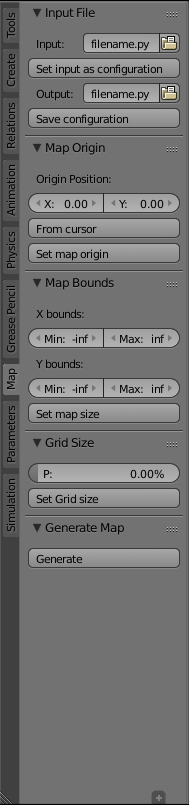
\includegraphics[height=10cm]{img/GUI_map_example.png}
    \caption{Map panel}
  \end{subfigure} % ~
  \begin{subfigure}[t]{0.2\textwidth}
    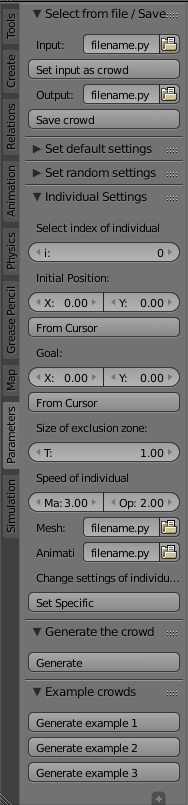
\includegraphics[height=10cm]{img/GUI_crowd_example.png}
    \caption{Crowd panel}
  \end{subfigure} % ~
  \begin{subfigure}[t]{0.5\textwidth}
    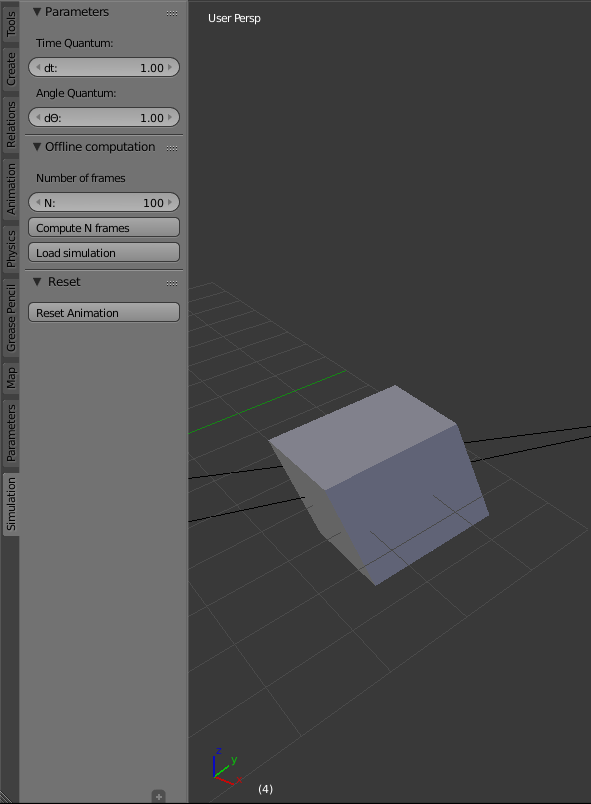
\includegraphics[height=10cm]{img/GUI_simulation_example.png}
    \caption{Simulation panel}
  \end{subfigure}
  \caption{The three panels of the GUI}
\end{figure}